This experiment tests how $\lambda$ controls the bias-variance trade-off. We scan $\lambda$ across a fixed grid. Figure~\ref{fig:lambda-sensitivity} tracks false positive rate, power, and effective sample size. Smaller $\lambda$ values more strongly correct weak-overlap bias but concentrate weights, lowering effective sample size. Larger values retain more sample mass but move the procedure toward the unweighted comparison. A moderate $\lambda$---around $0.5$ in these experiments---keeps the comparison focused on the common support while retaining enough sample mass to detect genuine harmful change.

\begin{figure}[t]
	\centering
	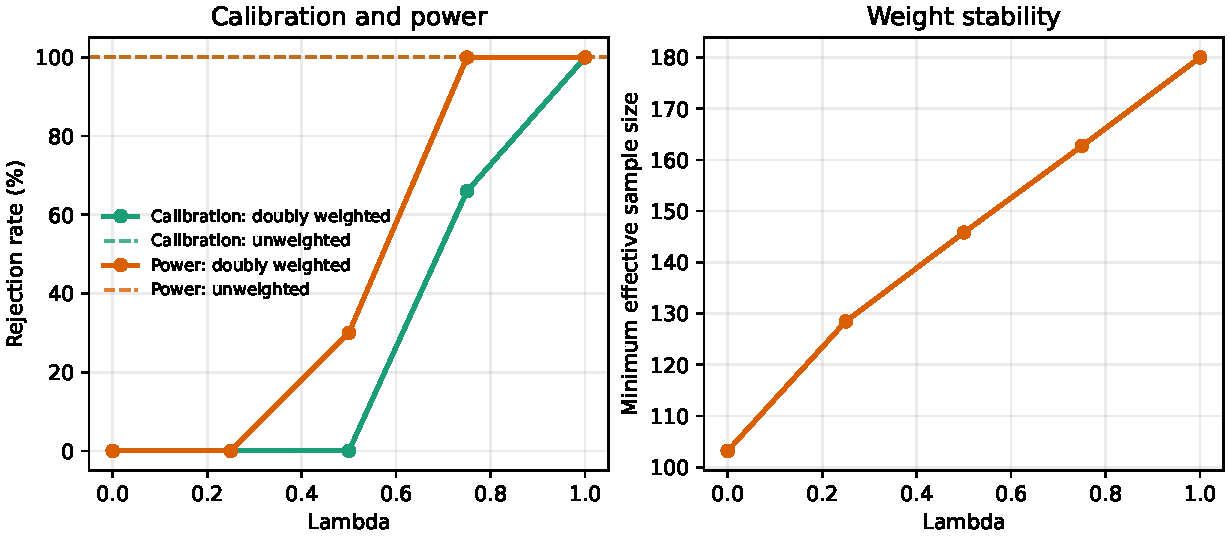
\includegraphics[width=0.98\linewidth]{figures/lambda_sensitivity_plot.pdf}
	\caption{Sensitivity to $\lambda$. Two-panel figure sharing the same x-axis ($\lambda$). Left panel (y-axis: rejection rate) shows calibration and power across $\lambda$ as solid lines for the doubly weighted mode, with horizontal dashed lines for the corresponding unweighted baseline. Right panel (y-axis: minimum effective sample size) tracks weight stability across the same $\lambda$ grid. Smaller $\lambda$ values correct weak-overlap bias more strongly but increase weight concentration. Larger values approach the unweighted regime.}
	\label{fig:lambda-sensitivity}
\end{figure}
